\section{Results}
\label{sec:results}
This chapter will present the results of the human detection and tracking system, including the system's performance in the museum environment, the effects of adding labeled images from the museum environment to the training dataset, and the system's ability to detect and track humans in real-time.

The FIMUS 2nd iteration images were used as the test set for all of the evaluations. This dataset consists of 295 images of similar light condition and image quality. They are the closest representation of the images the device will be capturing in the experimental setting. All images are of 3264x2464 resolution (which is the maximum for the hardware).

\subsection{Machine Learning Models of the Project}
The models in this project may be seen in table \ref{tab:performance_metrics}. All models were pre-trained with the COCO 2017 training/validation datasets. Unless stated otherwise, they all have image input sizes of 640. 

\subsubsection{YOLO}
The first 7 models are YOLOv9 models. 

The first three are fine-tuned with the FIMUS inconsistent dataset for respectively 5, 15 and 50 epochs while freezing the backbone\footnote{Freezing the backbone of a machine learning model is done to avoid unlearning basic shapes and features of the model. In transfer learning, this is a common practice when specializing a model to learn a new task or to better perform in a given sceneario where additional, specialized data may be limited.}. 

The fourth model is fine-tuned for 5 epochs on the CrowdHuman dataset, also with a frozen backbone. 

\paragraph{Input image size}
The fifth, sixth and seventh modelsare not fine-tuned. The dependent variable in this sub-experiment is the image size, which is the size of the input image when the model is performing inference. What input image size is optimal depends on the dataset and use case, and should be tested for a given sceneario. According to some, increasing the size may elevate the accuracy of a model (see the quote below). 

\begin{myquote}
	{Increasing the image size may elevate the accuracy of a model.}
	"We trained our model on images with a size of 640, which allows us to train a model with lesser computational resources. During inference, we increase the image size to 1280, allowing us to get more accurate results from our model" (\cite{ga2024roboflow_custom_dataset}).
\end{myquote}

In the experiment of this thesis, increasing the image size rendered worse results for the YOLOv9 model when considering the location accuracy of the detections as well. This discrepancy may be due to \citeauthor{ga2024roboflow_custom_dataset} only considering AP50, or it could be due to the difference in the datasets.

% The final YOLOv9 model serves as an illustration for how the scores would seem higher, were the detections calculated with a confidence threshold of .50 instead of .10. This is to artificially increase the AP50, AP75, AP90 and mAP50-95.  

The final YOLO model is a standard YOLOv3 model from Ultralytics.

\subsubsection{DETR}
The next models are built on the DETR architecture. The first uses a ResNet50 backbone, while the others use a ResNet101 backbone. The four last models are all 


\subsection{Model Evaluation}
The full model evaluation jupyter notebook can be seen in appendix todo insert model evaluation ipynb.

The confidence threshold for all detectors were set at 0.1, allowing for the calculation of an AP for confidence levels from 0.1 to 0.95. 

The FIMUS 5, 15 and 50 epochs are models pretuned on the COCO dataset, and fine-tuned with the FIMUS 1st iteration dataset. 

These were all trained for and detected at imgsz 640. The CrowdHuman 5 Epochs model was fine-tuned with 5 epocs on the training/validation datasets of CrowdHuman. The rest of the models were not fine-tuned.

\begin{table}[H]
    \centering
    \renewcommand{\arraystretch}{1.5} % Increase vertical padding
    \setlength{\tabcolsep}{1em}
    \begin{tabular}{|l|c|c|c|c|}
        \hline
        \rowcolor{gray!25}
        \textbf{Model} & \textbf{AP50} & \textbf{AP75} & \textbf{AP90} & \textbf{mAP50-95} \\ \hline
		FIMUS Fine-Tuned 5 Epochs              & 0\textbf{.97} & 0.89 & 0.67 & 0.88 \\ \hline
		FIMUS Fine-Tuned 15 Epochs             & 0.94 & 0.67 & 0.44 & 0.71 \\ \hline
		FIMUS Fine-Tuned 50 Epochs             & 0.94 & 0.75 & 0.51 & 0.77 \\ \hline
		CrowdHuman Fine-Tuned for 5 Epochs	   & 0.96 & 0.93 & 0.77 & 0.91 \\ \hline
		YOLOv9 Imagesize 320 		           & 0.92 & 0.85 & 0.62 & 0.84 \\ \hline
		YOLOv9 Imagesize 640 		           & 0.96 & 0\textbf{.93 & 0.90 & 0.94 }\\ \hline
		YOLOv9 Imagesize 1280		           & 0\textbf{.97} & 0.93 & 0.79 & 0.92 \\ \hline
		YOLOv3 							       & 0.95 & 0.88 & 0.63 & 0.87 \\ \hline
		DETR ResNet50					   	   & 0.32 & 0.29 & 0.17 & 0.28 \\ \hline	
		DETR ResNet101					       & 0.63 & 0.56 & 0.30 & 0.53 \\ \hline 
    \end{tabular}
    \caption{\centering Performance Metrics of Object Detection Models on 294 images.}
    \label{tab:performance_metrics}
\end{table}

% \begin{table}[H]
%     \centering
%     \renewcommand{\arraystretch}{1.5} % Increase vertical padding
%     \setlength{\tabcolsep}{1em}
%     \begin{tabular}{|l|c|c|c|c|}
%         \hline
%         \rowcolor{gray!25}
%         \textbf{Model} & \textbf{AP50} & \textbf{AP75} & \textbf{AP90} & \textbf{mAP50-95} \\ \hline
% 		DETR Confidence .90					   & 0.33 & 0.28 & 0.13 & 0.27 \\ \hline
% 		DETR Confidence .95					   & 0.98 & 0.87 & 0.41 & 0.83 \\ \hline
% 		DETR Confidence .97					   & \textbf{0.99} & 0.89 & 0.43	& 0.85 \\ \hline
% 		DETR Confidence .99					   & \textbf{0.99} & 0.92 & 0.48 & 0.88 \\ \hline
% 		Yolov9 Confidence .50				   & \textbf{0.99} & \textbf{0.97} & \textbf{0.95} & \textbf{0.98} \\ \hline
%     \end{tabular}
%     \caption{\centering Performance Metrics of Object Detection Models on 294 images.}
%     \label{tab:performance_metrics}
% \end{table}



\paragraph{Larger Test-set}
\phantomsection
\label{sec:larger_test_set}
As seen in table \ref{tab:larger_test_set}, adding in the images collected during the 3rd iteration reduced the scores for YOLOv9 while increasing the scores of the YOLOv3. The fact the scores change when adding more test data illustrates illustrate that we have not yet reached a level of test data where the scores converge. More test data should be added to further increase validity of the results.

\begin{table}[H]
    \centering
    \renewcommand{\arraystretch}{1.5} % Increase vertical padding
    \setlength{\tabcolsep}{1em}
    \begin{tabular}{|l|c|c|c|c|}
        \hline
        \rowcolor{gray!25}
        \textbf{Model} & \textbf{AP50} & \textbf{AP75} & \textbf{AP90} & \textbf{AP50-95} \\ \hline
		YOLOv3 (n=294) & 0.95 & 0.88 & 0.63 & 0.87 \\ \hline
		YOLOv3 (n=759) & 0.97 & 0.91 & 0.67 & 0.89 \\ \hline
		Yolov9 (n=294) & 0.99 & 0.97 & 0.95 & 0.98 \\ \hline
		YOLOv9 (n=759) & 0.98 & 0.96 & 0.93 & 0.96 \\ \hline
    \end{tabular}
    \caption{\centering Performance Metrics of Object Detection Models on 294 images vs 759 images}
    \label{tab:larger_test_set}
\end{table}

The pre-trained weights are available for multiple of the available versions of the Yolov9 model. The largest weights-file, called 'yolov9-e', is what has been used for this project. These weights are available for download on the \href{https://github.com/WongKinYiu/yolov9}{Yolov9 Github repository}.

\subsection{Data Visualization}
The data may be visualized a multiple of ways. The explored methods in this thesis are by creating heat maps and bar charts to visualize the data. 

\subsubsection{Heatmaps}
\label{sec:results_heatmaps}
As mentioned in section \ref{sec:heatmaps}, heatmaps are a powerful visualization tool that can provide insights into visitor behavior patterns and engagement levels within a museum or aquarium setting. Heatmaps for the month of may are illustrated in \ref{fig:heatmap_final}. These heatmap generation code for the two heatmaps are identical, apart from one variable: the position where detections are mapped to. In \ref{fig:heatmap_final}a and b, the detections are mapped to the respectively the middle and the bottom center of the detection bounding box. This single modification has the largest difference on the edges of occlusions, such as (for the images in figure \ref{fig:heatmap_final}) the railing of the fish tank in the center.

\begin{figure}[H]
    \centering
    \begin{subfigure}{0.475\textwidth}
        \centering
        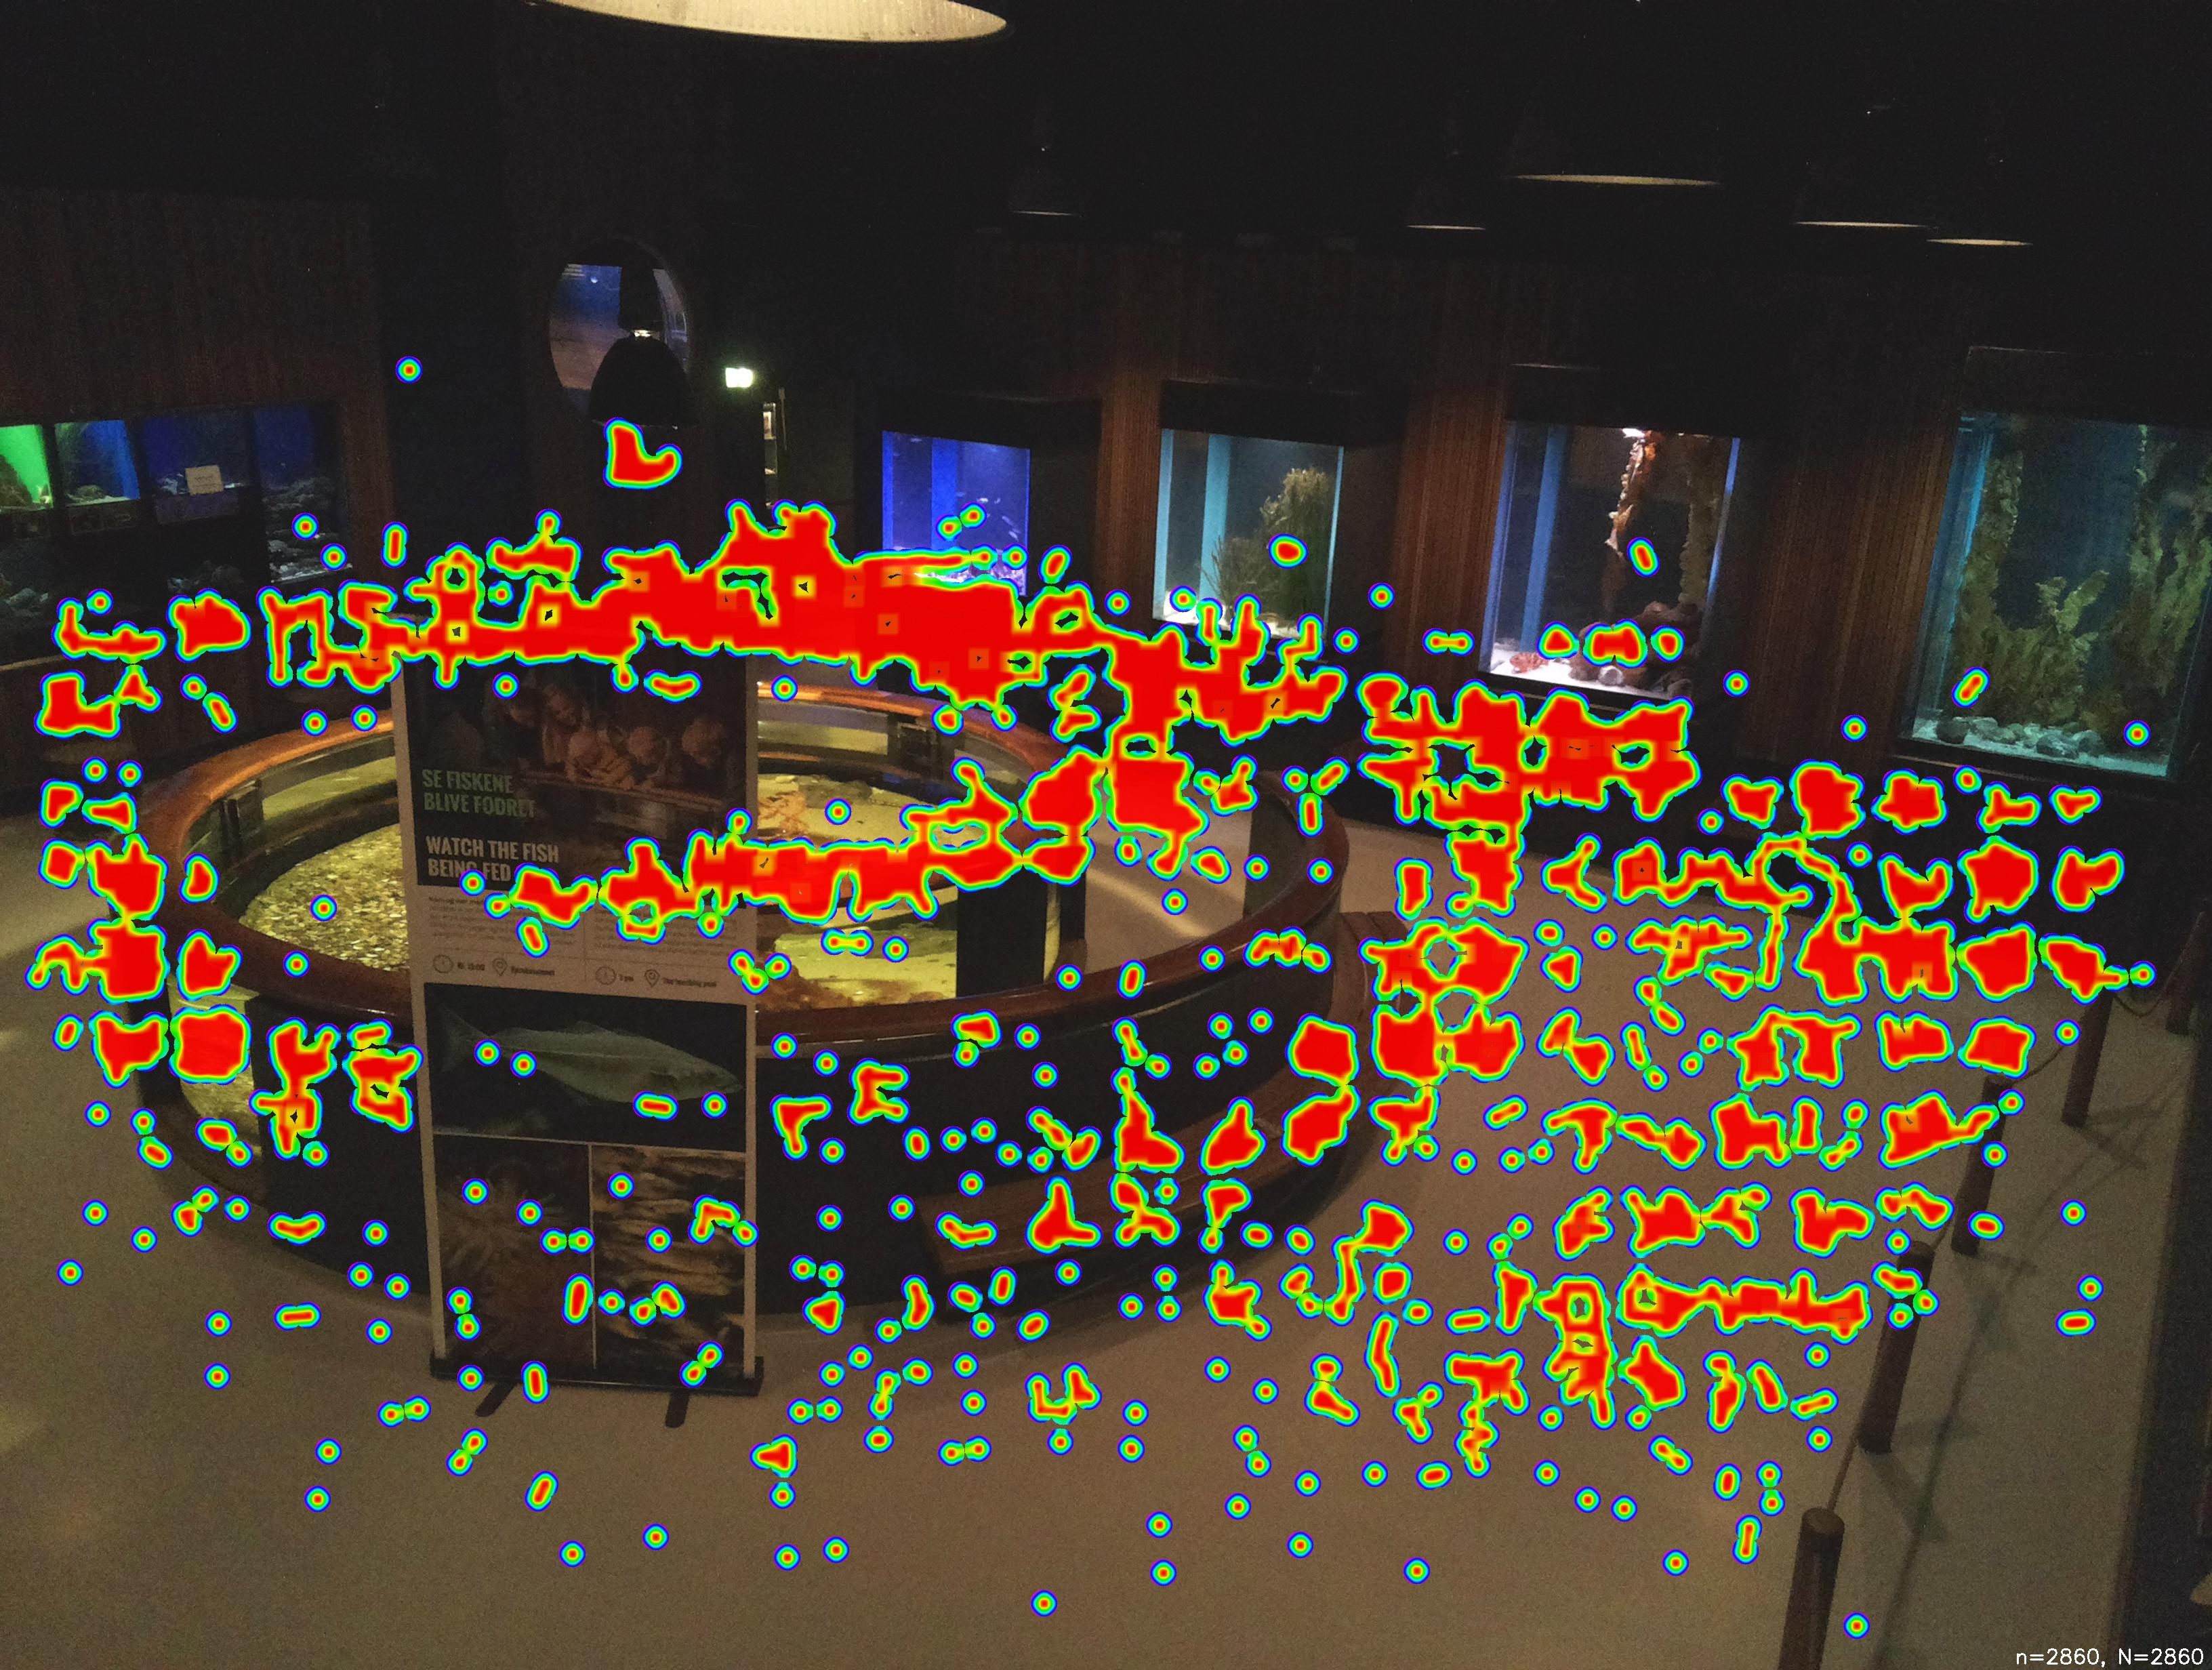
\includegraphics[width=\textwidth]{Images/Analytics/heatmap_supervision.jpg}
        \caption{Final Heatmap: Supervision, sampled from the \textit{middle} of detections}
    \end{subfigure}
    \hfill
    \begin{subfigure}{0.475\textwidth}
        \centering
        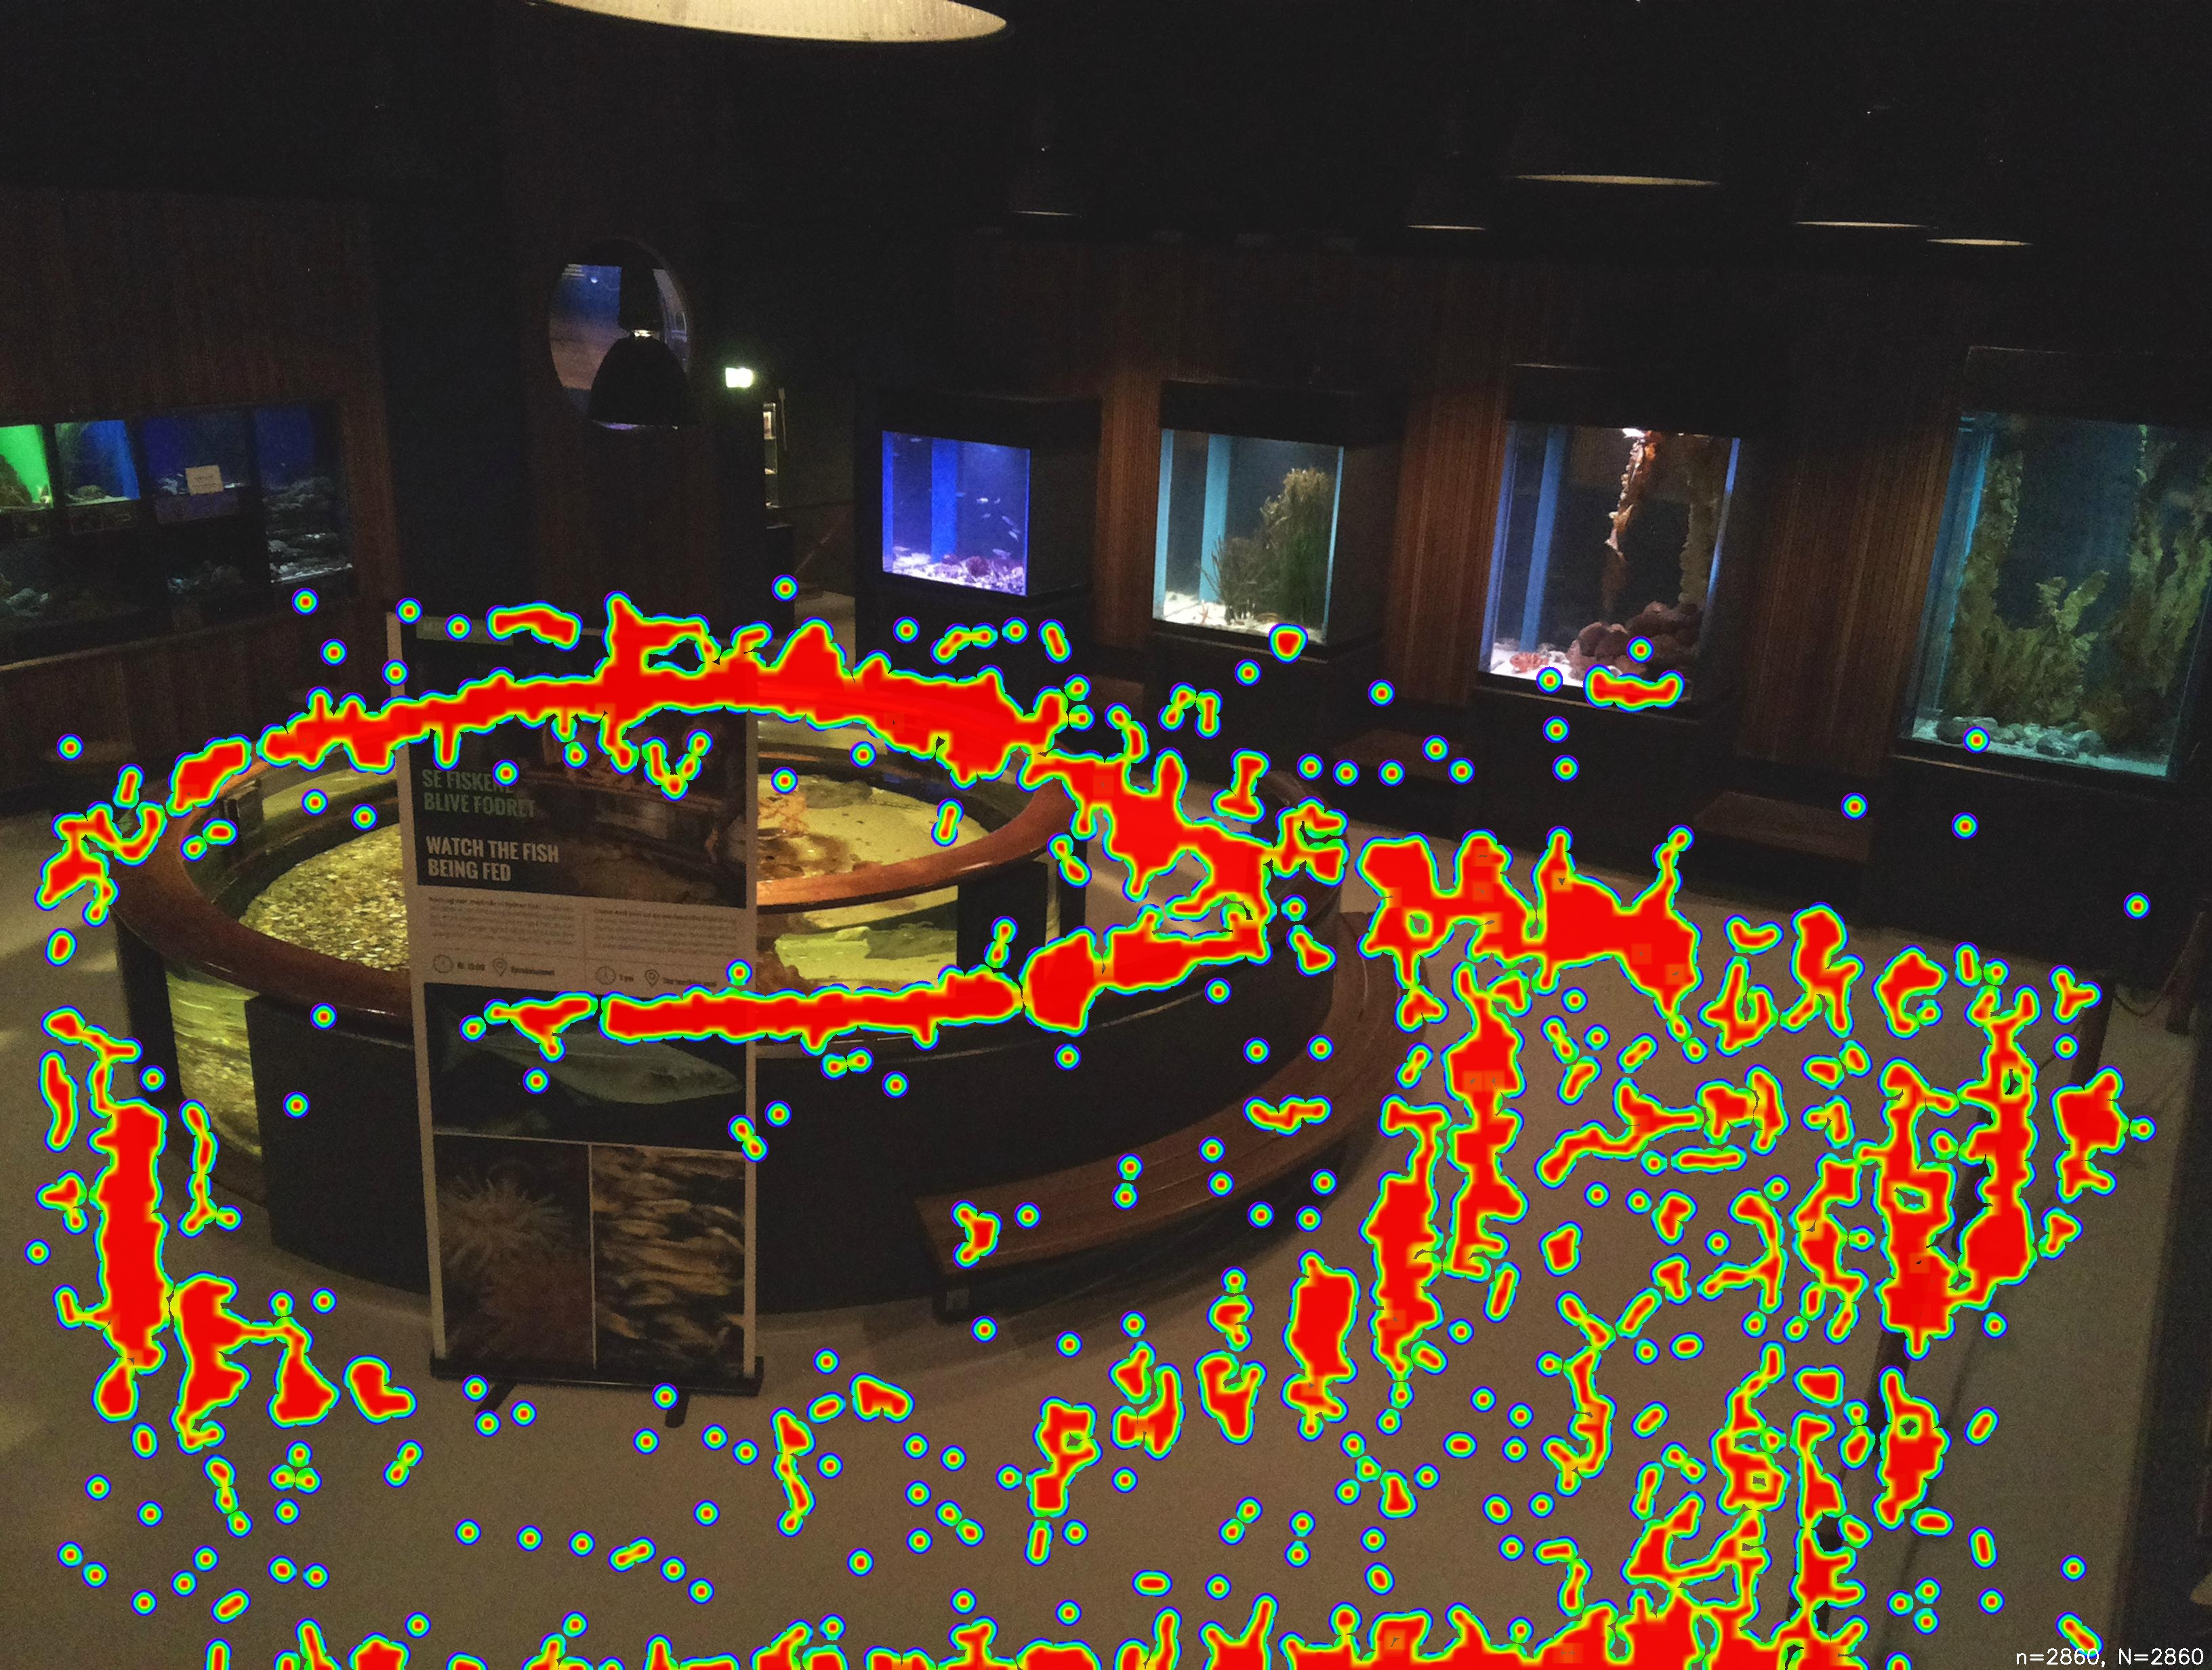
\includegraphics[width=1\textwidth]{Images/Analytics/heatmap_bottom_center.jpg}
        \caption{Final Heatmap: Supervision, sampled from the \textit{bottom} of detections}
    \end{subfigure}
    \caption{Final Heatmaps}
    \label{fig:heatmap_final}
\end{figure}

There's another, more important take away from the small modification. While seemingly similar, the heatmap sampling detections from the middle of the bounding boxes (\ref{fig:heatmap_final}a) reveal a weakness in our detector which is invisible in the other heatmap: the lamp is sometimes classified as a person. On the other hand, the other heatmap (\ref{fig:heatmap_final}b) reveal another weakness. The seaweed in the second fish tank from the right is sometimes also classified as a person.   

Apart from revealing weaknesses from the detector models\footnote{These weaknesses in our detector models could be revealed by looking at the annotated images. However, looking at the annotated images is not possible for a on-device processing image-deleting device. In this case, one would need to display/plot the detections onto a base-layer image (heat map), or make use of obfuscation discussed in section \ref{sec:obfuscation} to illustrate and reveal model weaknesses.}, these heatmaps may provide valuable insights with regards to which areas of the facility are being used the most. There may be difficulties, however, in correctly inferring what are the reasons for the variations. For periods less than a day, these variations are likely due to randomness. The more interesting numbers in this context would be to see the total number of visitors throughout the day, which is better visualized in the bar charts in section \ref{sec:peak_hours}. Two heatmaps for separate days are illustrated in figure \ref{fig:heatmap_daily}.

\begin{figure}[H]
    \centering
    \begin{subfigure}{0.475\textwidth}
        \centering
        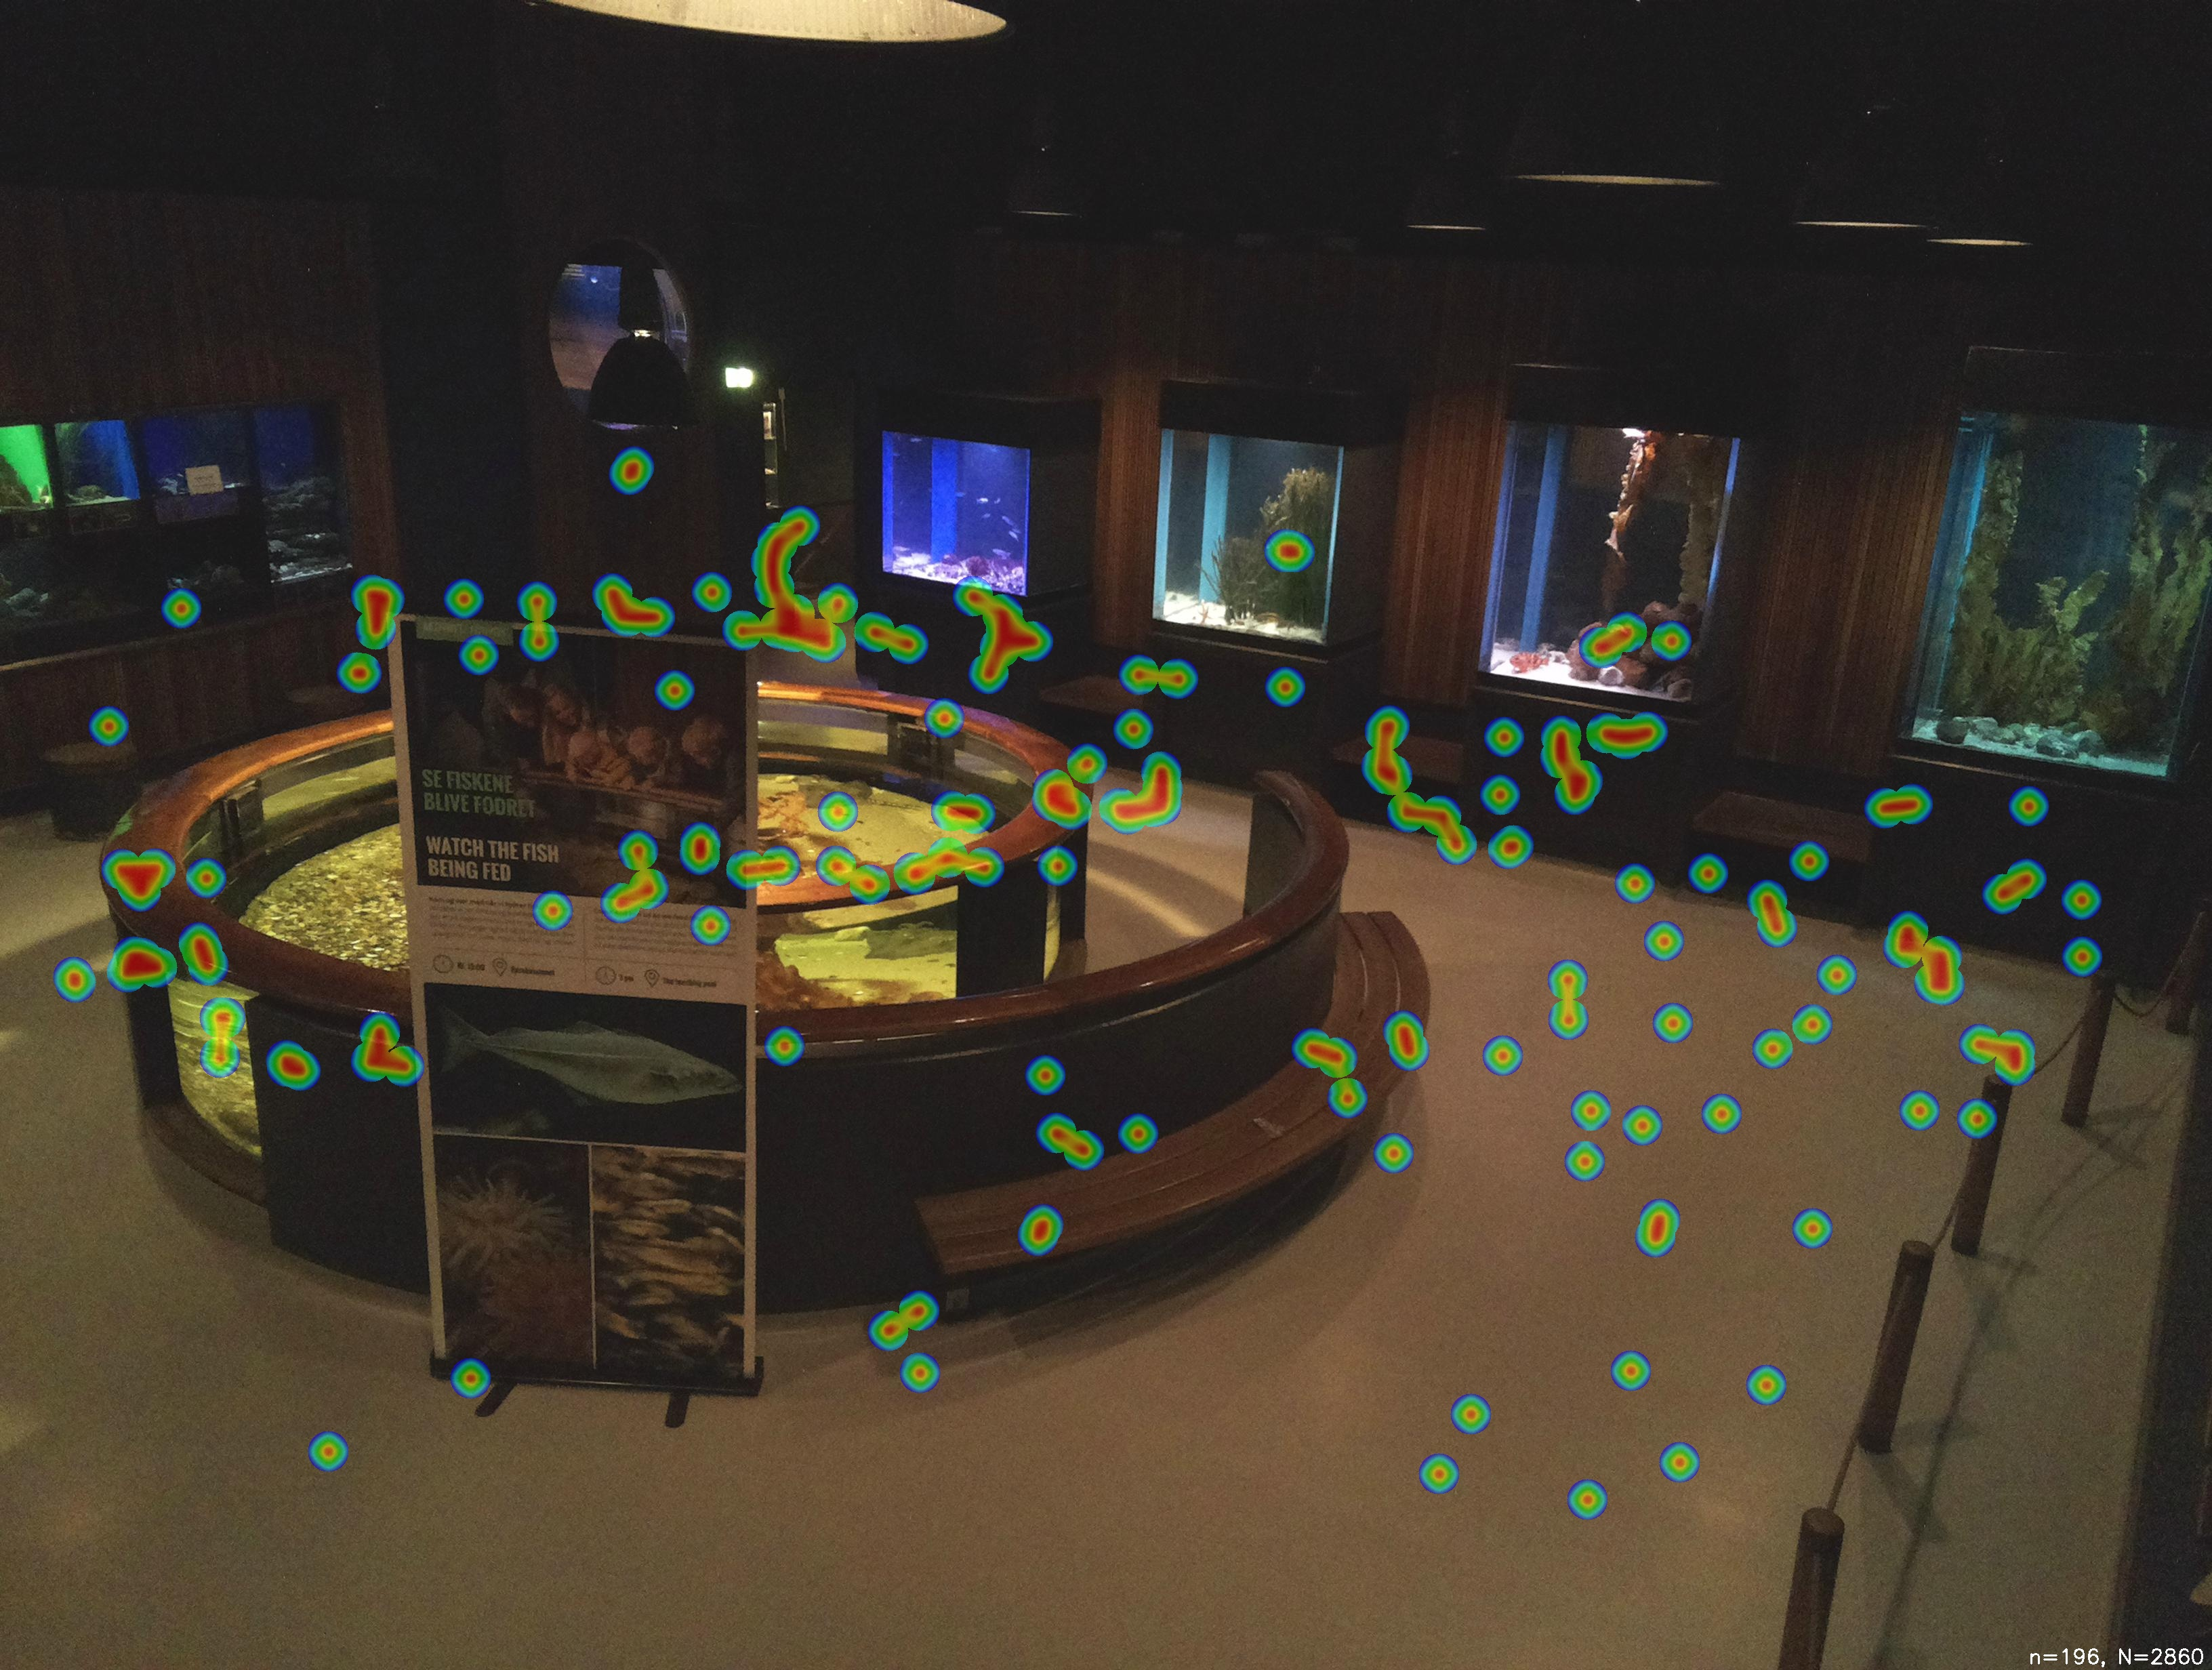
\includegraphics[width=\textwidth]{Images/Analytics/heatmap_day_08052024.jpg}
        \caption{Heatmap Wednesday 8th of May, 2024}
    \end{subfigure}
    \hfill
    \begin{subfigure}{0.475\textwidth}
        \centering
        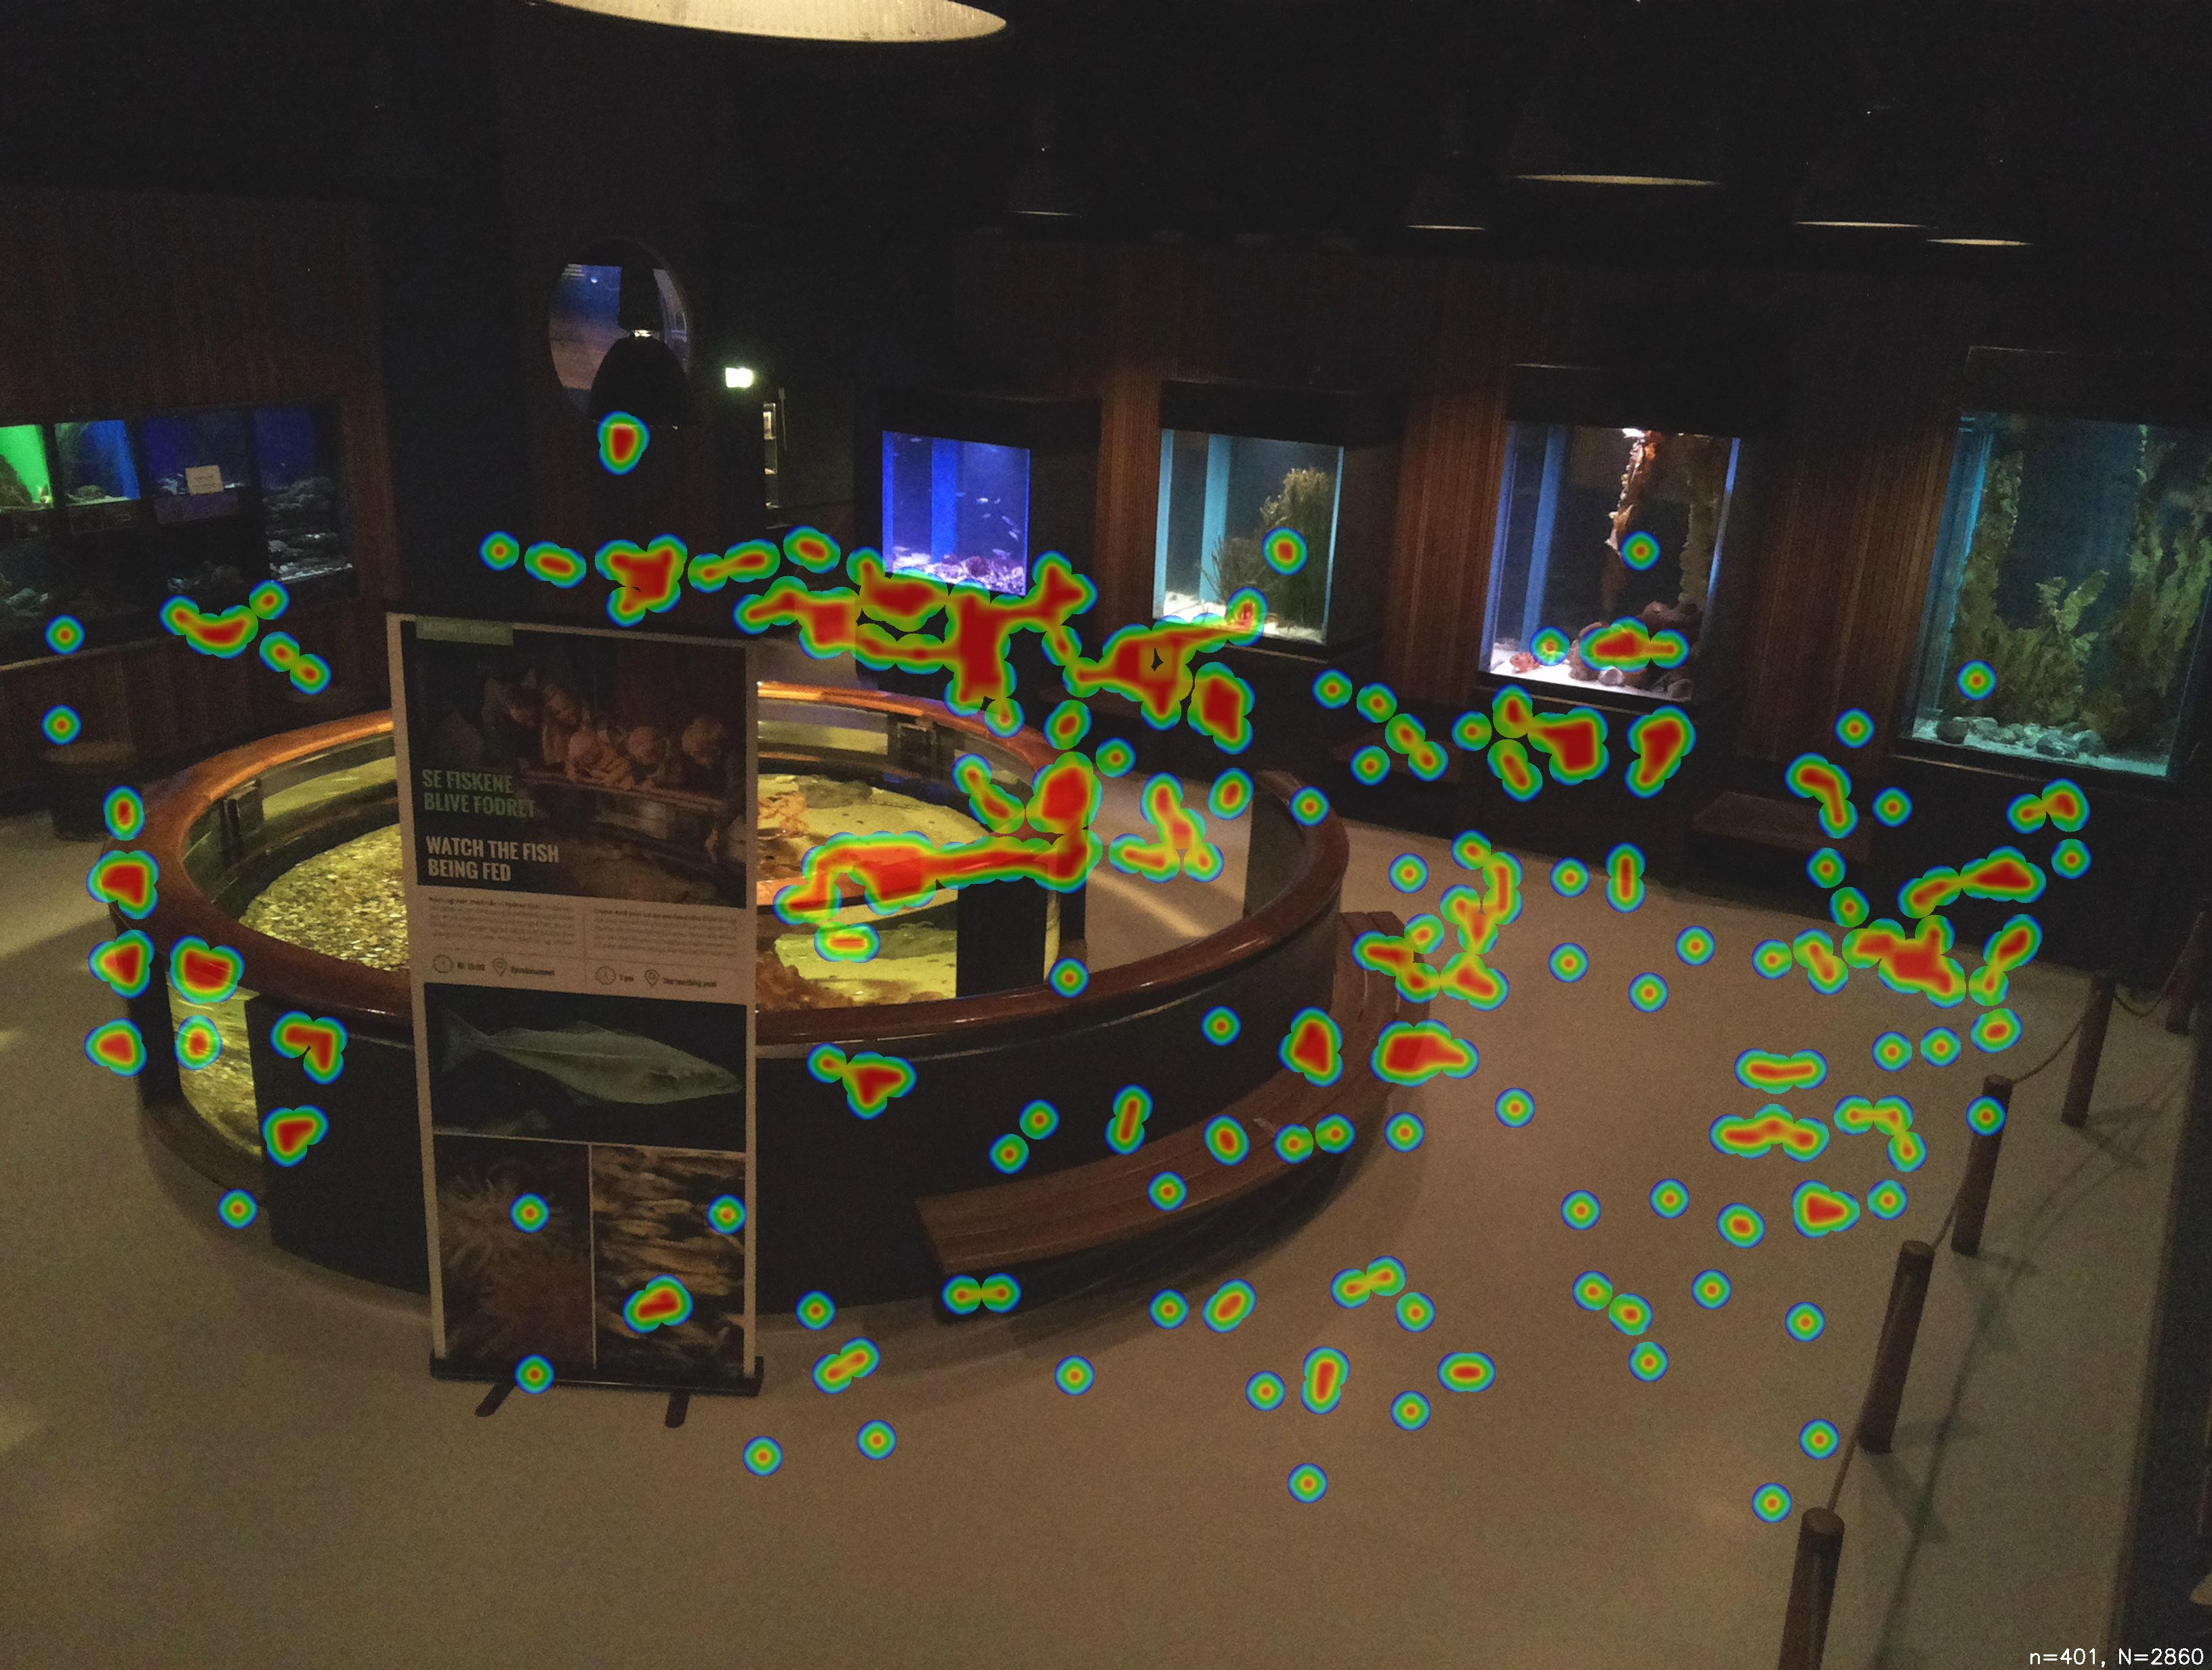
\includegraphics[width=1\textwidth]{Images/Analytics/heatmap_day_11052024.jpg}
        \caption{Heatmap Saturday 11th of May, 2024}
    \end{subfigure}
    \caption{Daily Heatmap}
    \label{fig:heatmap_daily}
\end{figure}

Heat maps may also visualize the hours throughout a day, accumulating all data for a specific time period each day to see if the visitor engagement changes based on the time. This is one example of introducing a variable, namely the time of day, to filter the detections. For an area where other variables such as the temperature, the noise level or the weather is also known, this could be used instead to filter the detections and illustrate how visitor engagement changes based on these factors. This usage would naturally, require some months-worth of data to be valid. For this project, only a months-worth of localization data has been stored to make the analysis. An illustration of heatmaps where the time of day has been used to determine which detections are presented in the heatmaps are displayed in figure \ref{fig:heatmap_time}.

\begin{figure}[H]
    \centering
    \begin{subfigure}{0.475\textwidth}
        \centering
        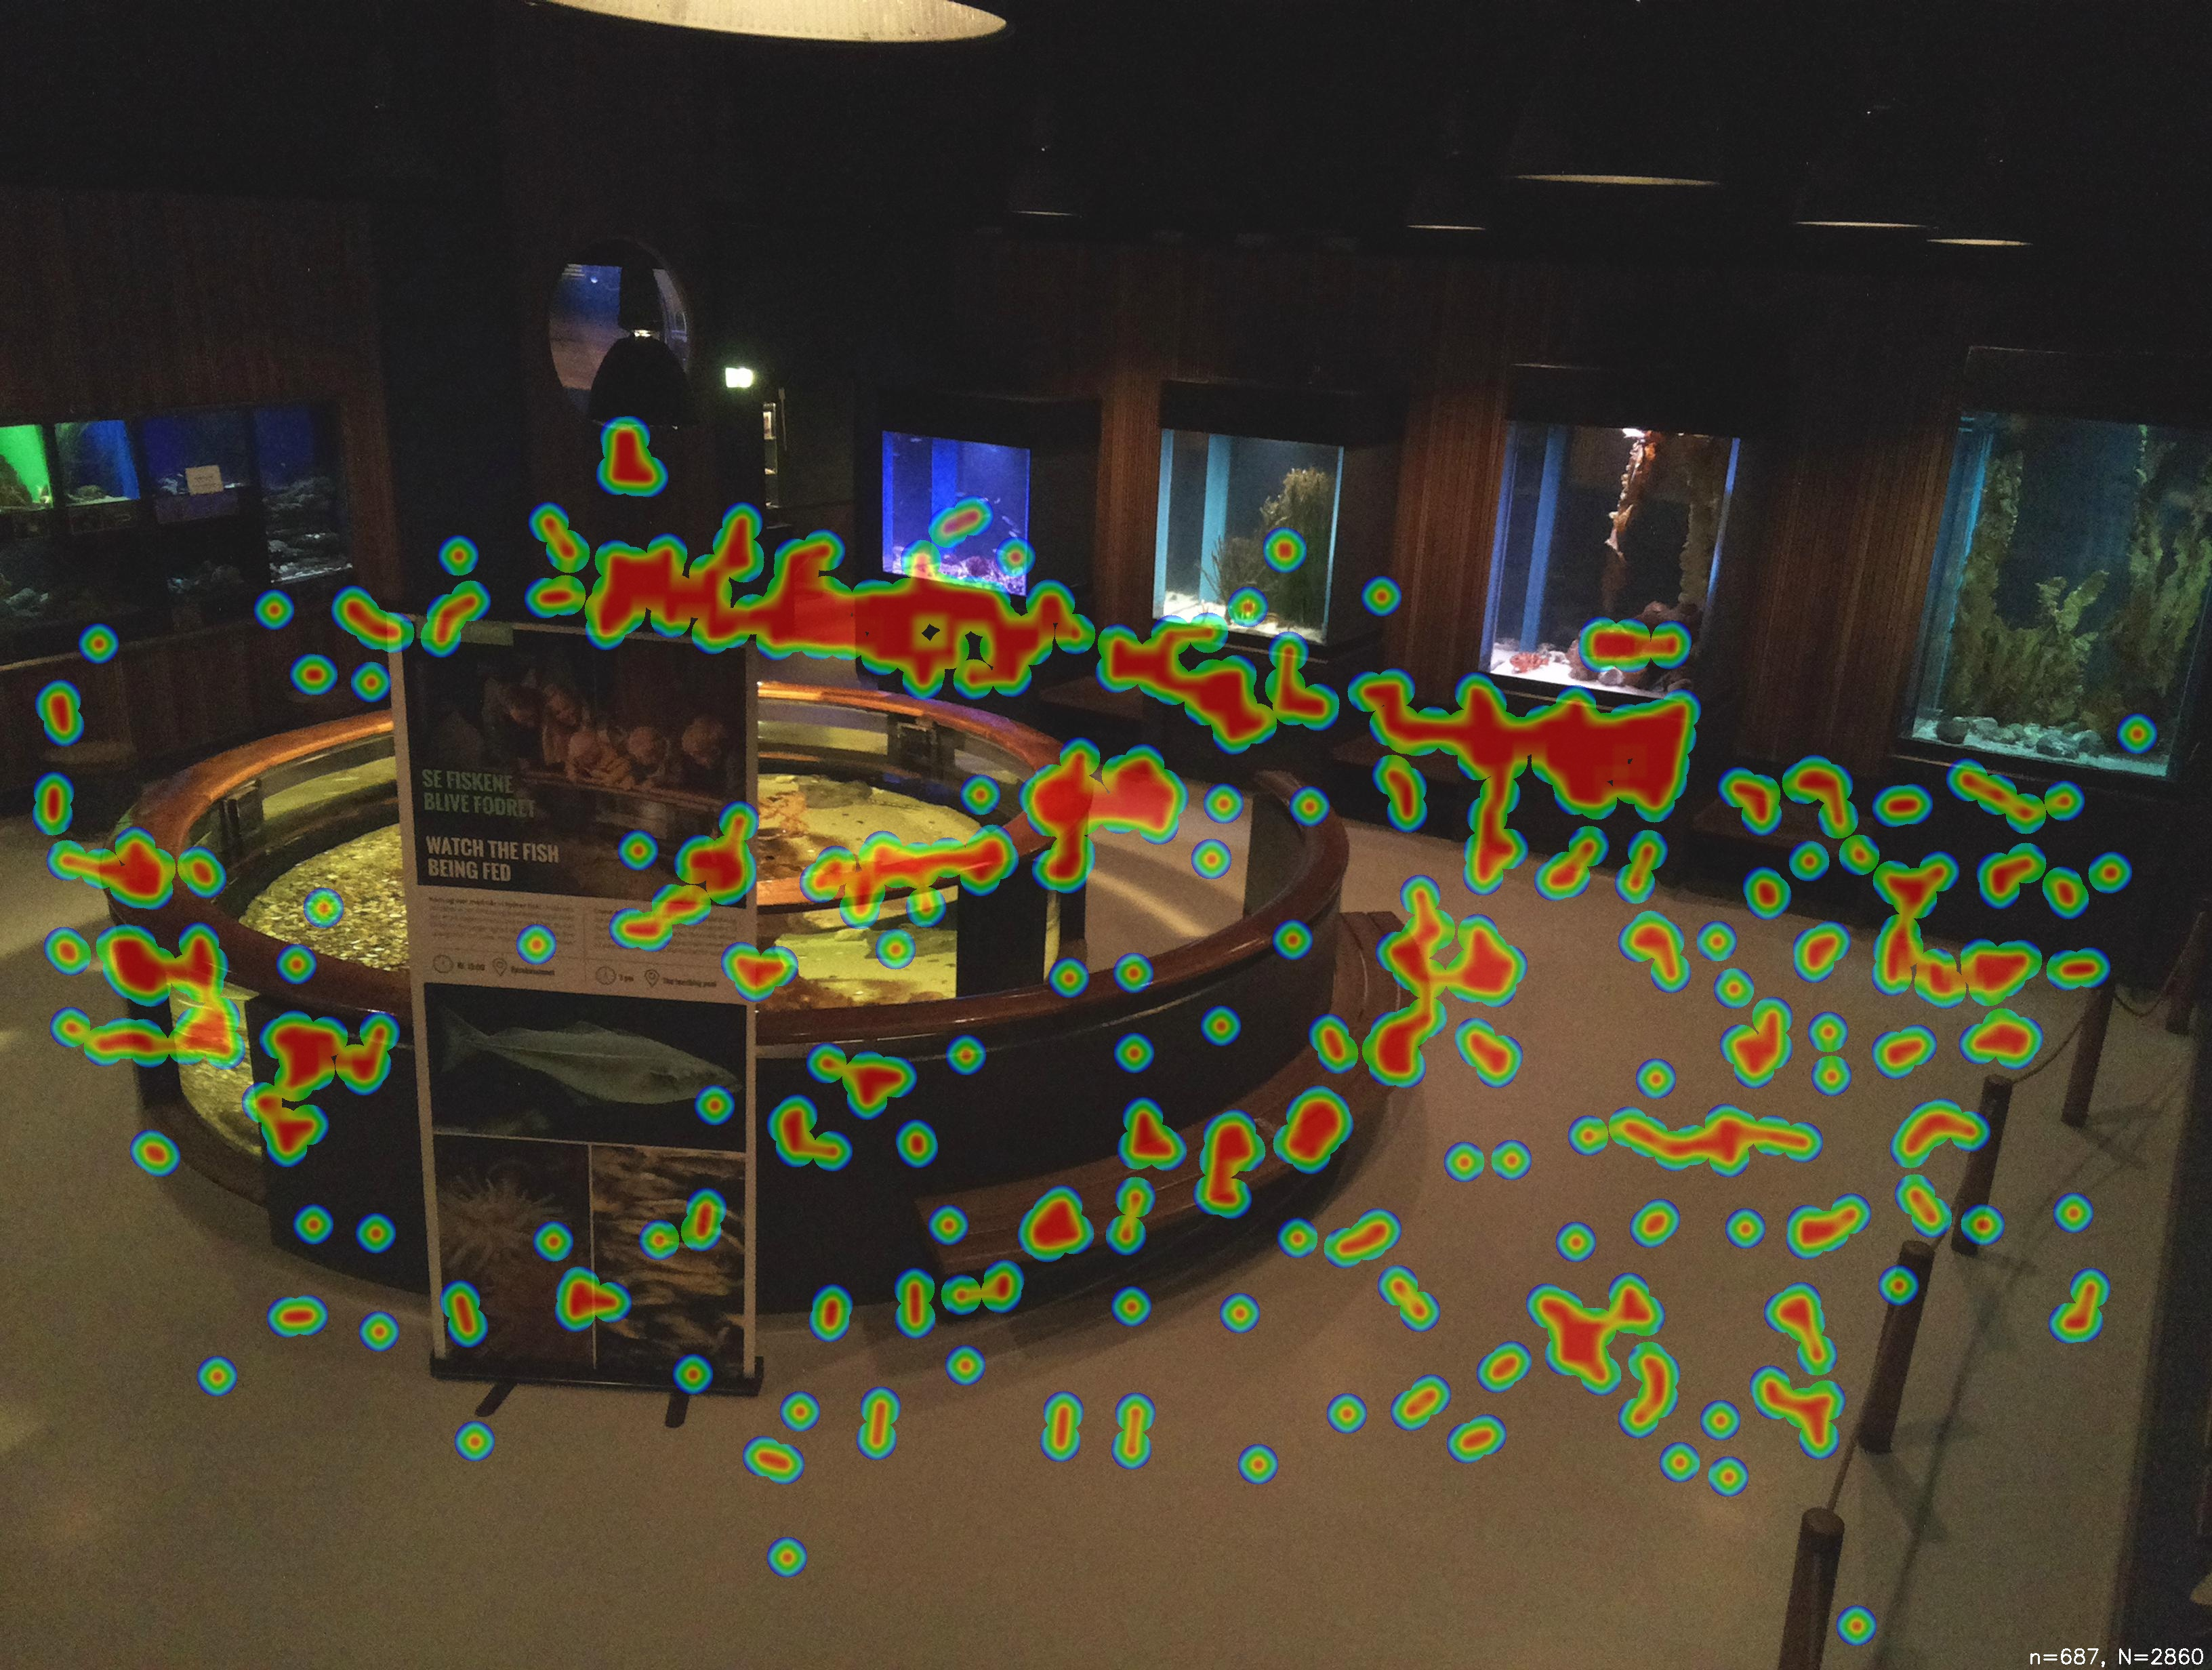
\includegraphics[width=\textwidth]{Images/Analytics/heatmap_time_1300_1400.jpg}
        \caption{Heatmap 13:00-14:00}
    \end{subfigure}
    \hfill
    \begin{subfigure}{0.475\textwidth}
        \centering
        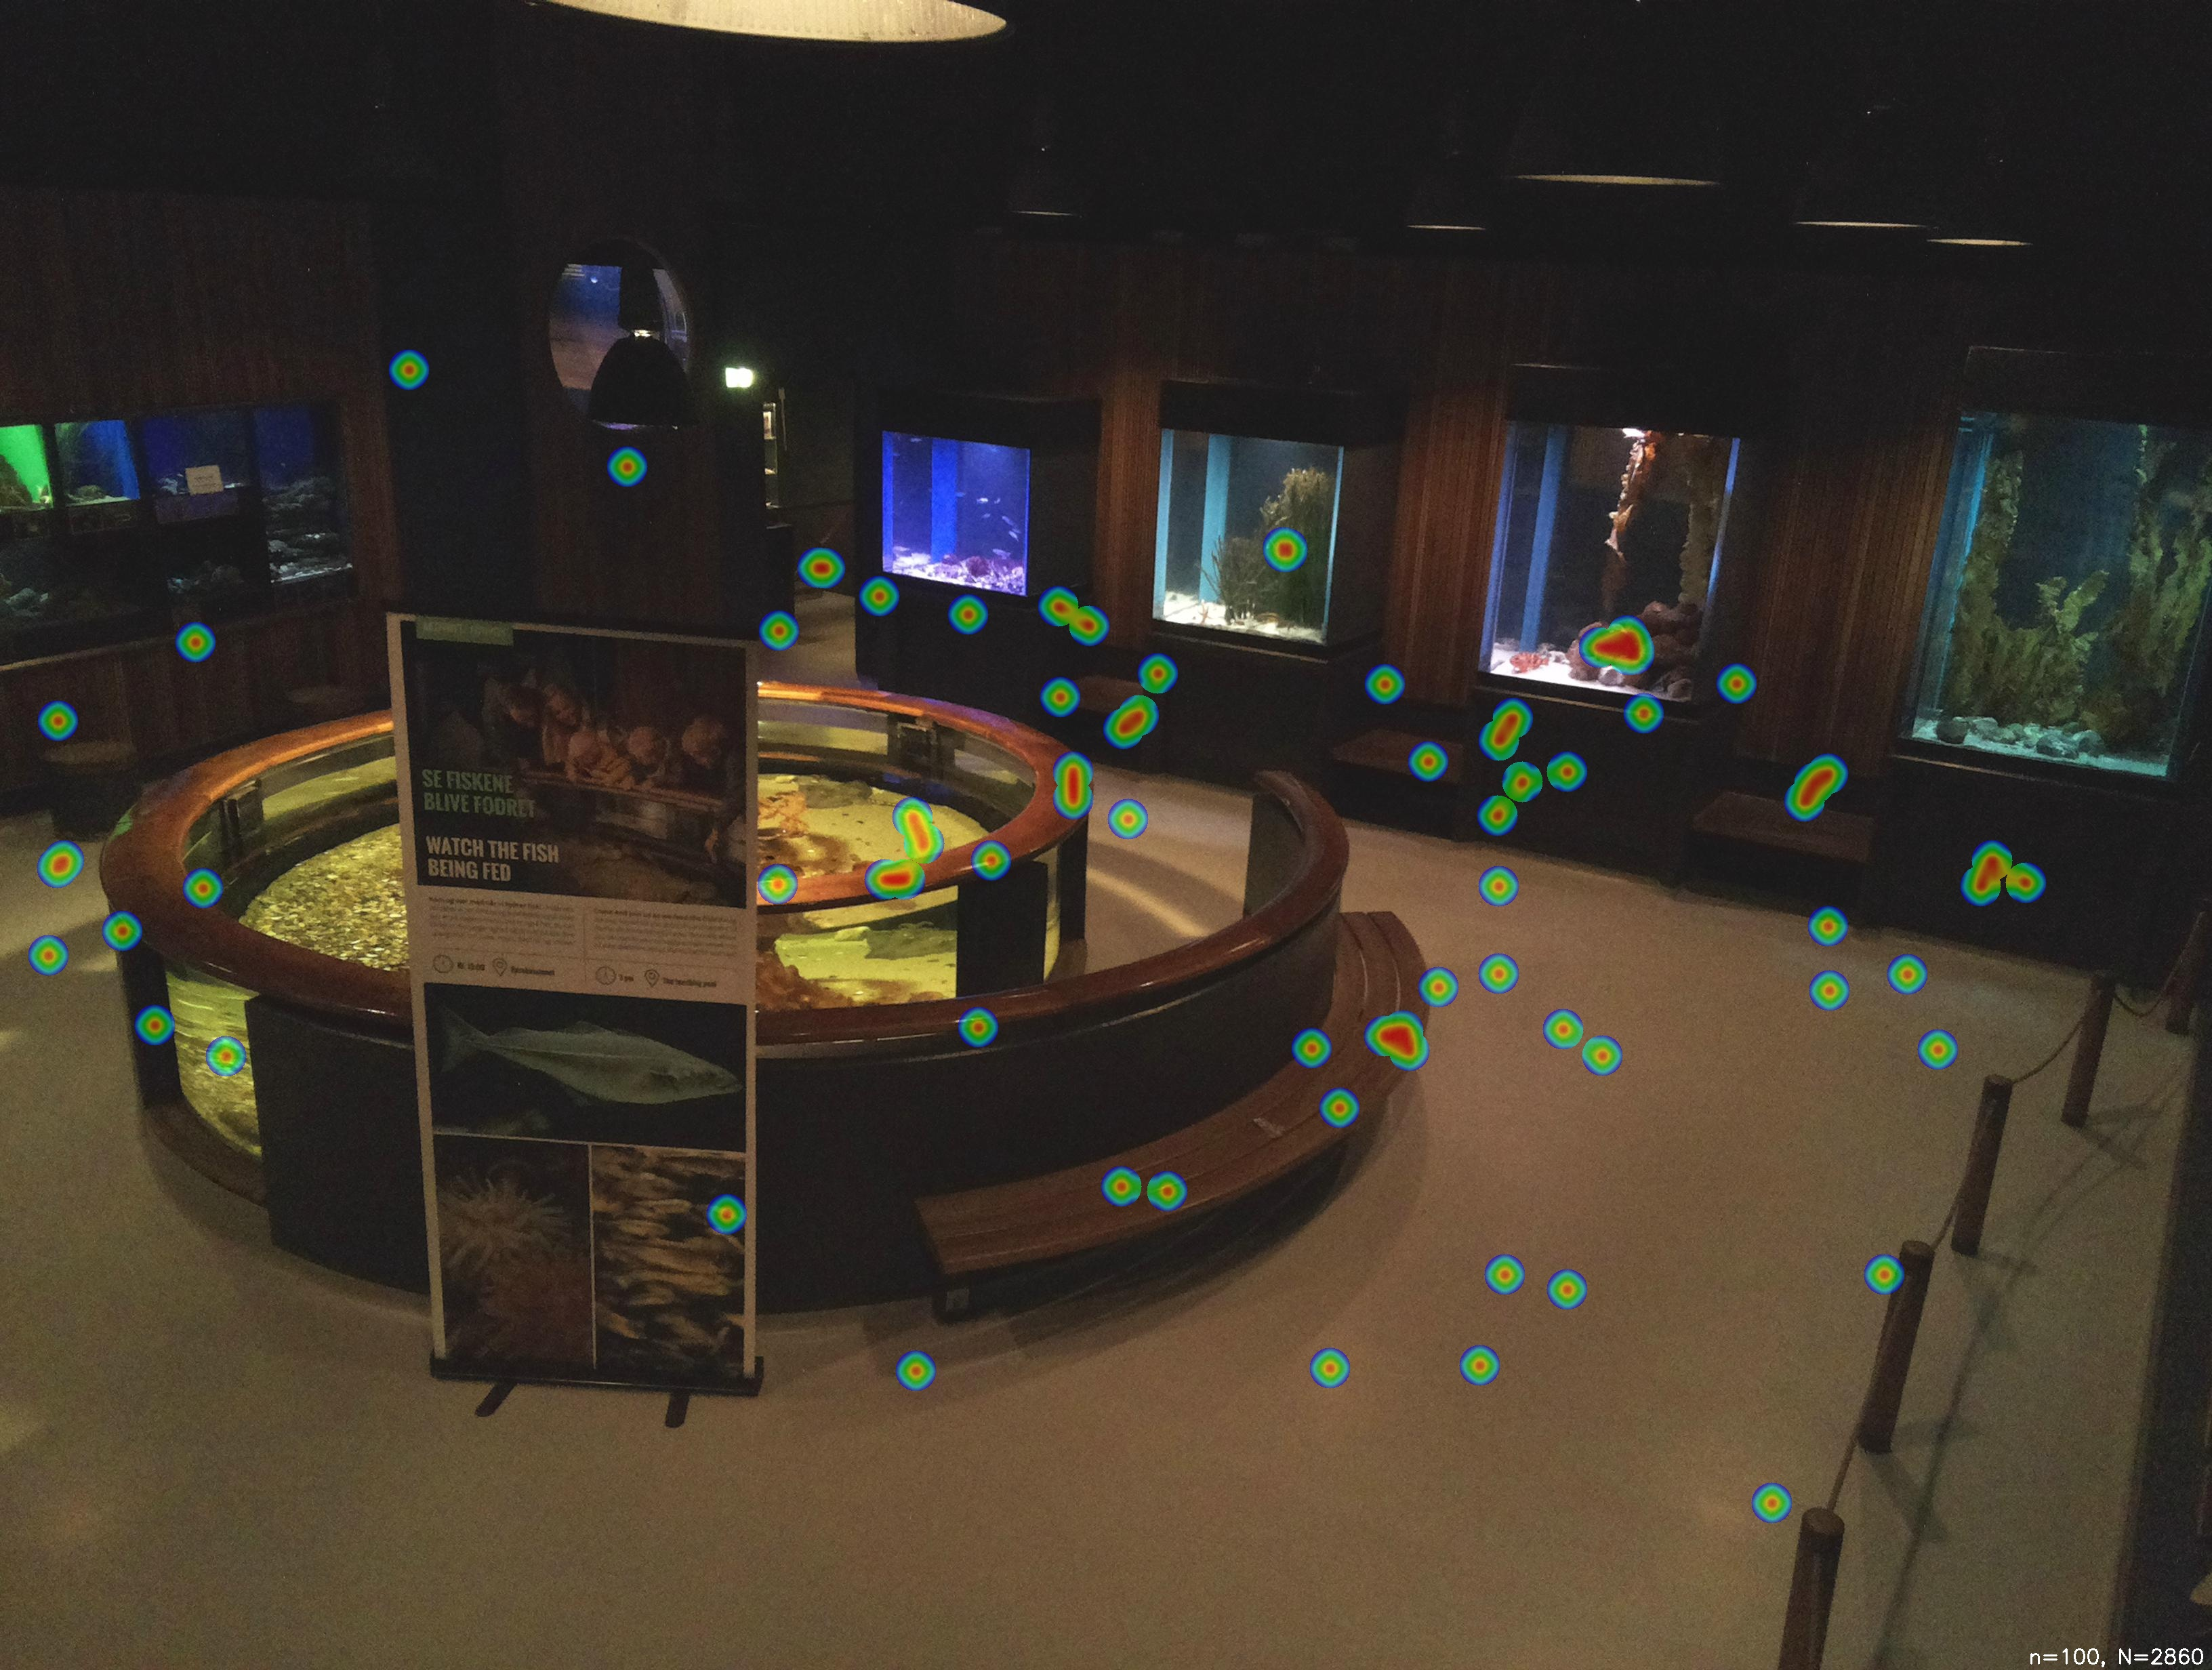
\includegraphics[width=1\textwidth]{Images/Analytics/heatmap_time_1600_1700.jpg}
        \caption{Heatmap 16:00-17:00}
    \end{subfigure}
    \caption{Hourly Heatmap}
    \label{fig:heatmap_time}
\end{figure}

The heatmaps in figure \ref{fig:heatmap_time} reveal another use case for heatmaps. The relative difference between the two heatmaps is likely due to randomness, but with a larger number of detections one might be able to look for patterns. This could be that the heatmap for 13:00-14:00 could show a higher number of detections in front of the fish tanks, while the heatmap for 16:00-17:00 could show a higher number of detections on the benches. This could have easily been overlooked, had a manager of the museum only passed through the museum in the day and never in the evenings, resulting in him not thinking so many benches were neccessary. 



\subsubsection{Peak Hours}
\label{sec:peak_hours}
Another tool is to analyze the average number of detected persons per hour. This provides insights into room utilization during different times of the day.

\begin{figure}[H]
	\centering
	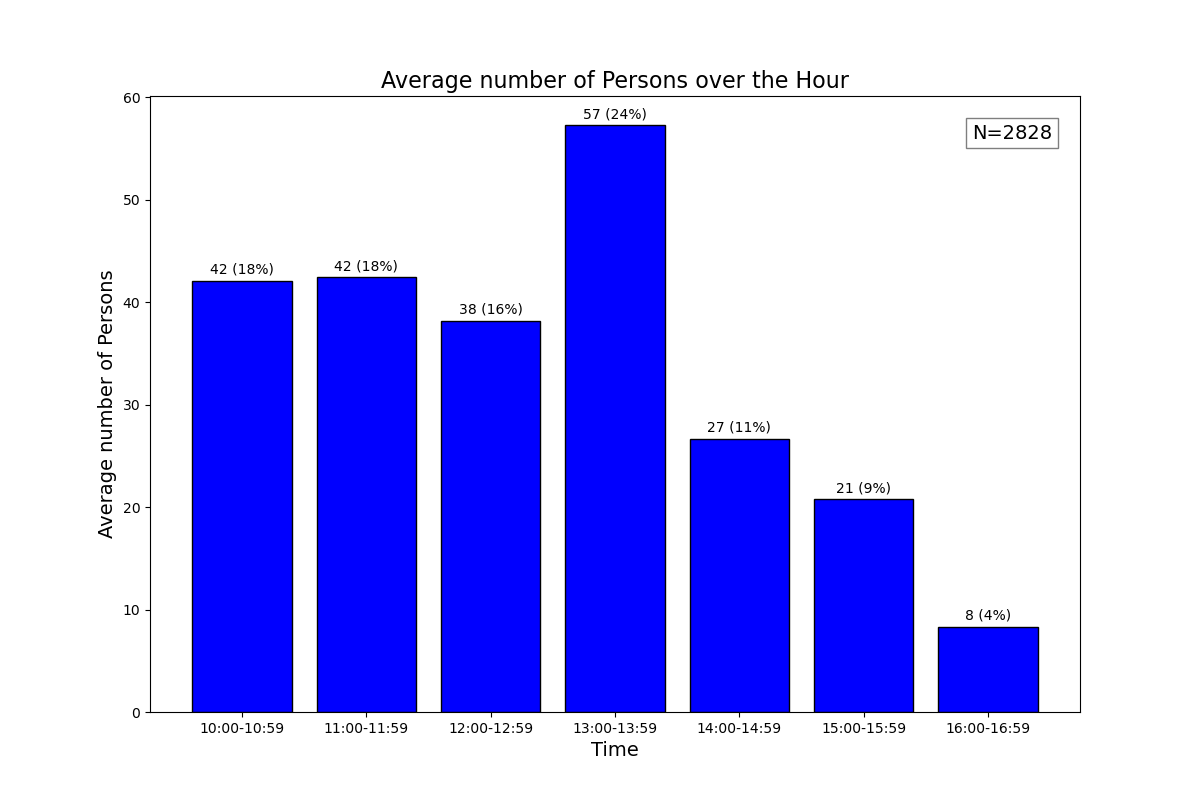
\includegraphics[width=1\textwidth]{Images/Analytics/peak_hours.png}
	\caption{Peak Hours Analysis}
    \label{fig:peak_hours}
\end{figure}

For instance, a lower number of detections during early opening hours, despite high visitor entry, could indicate that the room temperature is not yet optimal, affecting visitor comfort. This hypothesis could be tested by using the number of visitors as the dependent variable and adjust the room temperature to see the effects. In the absence of other confounding variables\footnote{Which may be a difficult and nearly impossible task in a real-world setting. Altough providing high ecological validity, such a setting makes it nearly impossible to infer valid results due to the high chance of unforeseen or even random events affecting the results.}, this could be an interesting causal relationsship to investigate to infer the perfect room temperature. However, due to the requirement in such an investigation for the high volume of data to rule out the possibility of randomness confounding the results, this investigation is likely unrealistic.

Further, comparing visitor detections of summer vs winter months, normalized for the total visitors in the facility, could provide deeper insights. It would enable the possibility of gauging the relative popularity of different areas. Indoor environments, typically maintained at constant temperatures, might offer different levels of comfort compared to the naturally fluctuating conditions of outdoor areas. 

Understanding these dynamics can guide decisions on environmental controls, such as adjusting heating levels to enhance visitor comfort and potentially increase engagement in specific areas of the facility. Such adjustments could directly influence the overall visitation experience, making the whole facility more favorable for a visit regardless of seasonal factors.


\subsection{Third-party Services}
\label{sec:discuss_thirdparty}
As we've seen in section \ref{sec:thirdparty}, third-party services offer convenient solutions that may align perfectly with specific requirements for object detection systems, providing a quick and efficient path to implementation. There are potential drawbacks, however. These are listed below.

\subsubsection{Drawbacks of Utilizing Third-Party Services}
\begin{enumerate}
    \item \textbf{Complete Control Over the System:} Developing your own application allows for full customization in terms of software architecture, data processing, and system integration. This total control facilitates the optimization of the system to meet specific performance and operational requirements. In addition, a system built separately would have the benefit of being independent from the performance and existence of Roboflow.
    \item \textbf{Data Privacy and Security:} On-device processing ensures that all data processing is kept on-device, enhancing data security and privacy. Roboflow offers local deployment, but this comes as part of their more expensive business-level subsxription plan.
    \item \textbf{Cost Efficiency:} Managing your own system can be more cost-effective in the long run, particularly if the application demands extensive processing power or high throughput, as it eliminates recurring costs associated with third-party platforms. Roboflow's plans include costs related to "inference credits", making the system great for small applications but less likely to be a good fit for bigger enterprise solutions looking to leverage the margins. GPT4-V may be accessed via Azure's OpenAI service, which is also priced by how much the service is used and how
    \item \textbf{Performance Optimization:} Owning the inference system allows for hardware and software optimizations that are not possible when using third-party services. This can lead to better performance, especially in terms of processing speed and latency.
    \item \textbf{Scalability and Integration Flexibility:} Implementing your own solution allows for easier scaling and integration with existing IT infrastructure, which is beneficial for maintaining seamless data workflows and supporting business growth without being limited by external platform constraints.
\end{enumerate}

While leveraging third-party services can expedite development, it is imperative for researchers and practitioners in the field of object detection, particularly in contexts such as person detection where privacy may be of cencern, to carefully weigh these considerations. Exploring alternative methods of implementation, including developing systems from scratch, can offer greater flexibility, control, and potential for innovation.

